\documentclass[../../main.tex]{subfiles}
\graphicspath{{\subfix{../../image/}}} % 指定图片目录,后续可以直接使用图片文件名。

% 例如:
% \begin{figure}[H]
% \centering
% \includegraphics[scale=0.4]{图.png}
% \caption{}
% \label{figure:图}
% \end{figure}
% 注意:上述\label{}一定要放在\caption{}之后,否则引用图片序号会只会显示??.

\begin{document}

\section{分段低次插值}

\subsection{高次插值的病态性质}\label{高次插值导致的龙格现象}

上面我们根据区间 $[a, b]$ 上给出的节点做插值多项式 $L_n(x)$ 近似 $f(x)$, 一般总认为 $L_n(x)$ 的次数 $n$ 越高逼近 $f(x)$ 的精度越好, 但实际上并非如此. 这是因为对任意的插值节点, 当 $n \to \infty$ 时, $L_n(x)$ 不一定收敛于 $f(x)$. 20 世纪初龙格 (Runge) 就给出了一个等距节点插值多项式 $L_n(x)$ 不收敛于 $f(x)$ 的例子. 他给出的函数为 $f(x) = 1/(1 + x^2)$, 它在 $[-5, 5]$ 上各阶导数均存在. 在 $[-5, 5]$ 上取 $n + 1$ 个等距节点 $x_k = -5 + 10 \frac{k}{n}$ ($k = 0, 1, \cdots, n$) 所构造的拉格朗日插值多项式为
\[
L_n(x) = \sum_{j=0}^n \frac{1}{1 + x_j^2} \frac{\omega_{n+1}(x)}{(x - x_j) \omega_{n+1}'(x_j)}.
\]
令 $x_{n - 1/2} = \frac{1}{2}(x_{n - 1} + x_n)$, 则 $x_{n - 1/2} = 5 - \frac{5}{n}$, 表 2-5 列出了当 $n = 2, 4, \cdots, 20$ 时的 $L_n(x_{n - 1/2})$ 的计算结果及在 $x_{n - 1/2}$ 上的误差 $R(x_{n - 1/2})$. 可以看出, 随着 $n$ 的增加, $R(x_{n - 1/2})$ 的绝对值几乎成倍地增加. 这说明当 $n \to \infty$ 时, $L_n$ 在 $[-5, 5]$ 上不收敛. 龙格证明了, 存在一个常数 $c \approx 3.63$, 使得当 $|x| \leqslant c$ 时, $\lim\limits_{n \to \infty} L_n(x) = f(x)$, 而当 $|x| > c$ 时 $\{L_n(x)\}$ 发散.
\begin{table}[H]
\centering
\caption{计算结果及误差}
\begin{tabular}{c|c|c|c}
\toprule
$n$ & $f(x_{n - 1/2})$ & $L_n(x_{n - 1/2})$ & $R(x_{n - 1/2})$ \\
\midrule
2  & 0.137931 & 0.759615   & -0.621684  \\
4  & 0.066390 & -0.356826  & 0.423216   \\
6  & 0.054463 & 0.607879   & -0.553416  \\
8  & 0.049651 & -0.831017  & 0.880668   \\
10 & 0.047059 & 1.578721   & -1.531662  \\
12 & 0.045440 & -2.755000  & 2.800440   \\
14 & 0.044334 & 5.332743   & -5.288409 \\
16 & 0.043530 & -10.173867 & 10.217397  \\
18 & 0.042920 & 20.123671  & -20.080751 \\
20 & 0.042440 & -39.952449 & 39.994889  \\
\bottomrule
\end{tabular}
\end{table}
下面取 $n = 10$, 根据计算画出 $y = L_{10}(x)$ 及 $y = 1/(1 + x^2)$ 在 $[-5, 5]$ 上的图形, 见\reffig{figure:高次插值的龙格现象}.
\begin{figure}[H]
\centering
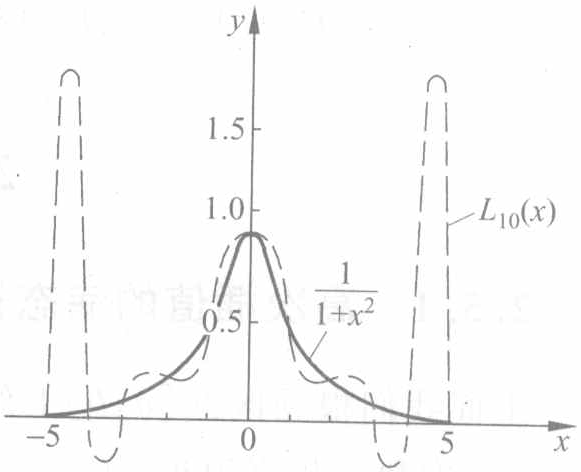
\includegraphics[scale=0.4]{高次插值的龙格现象.png}
\caption{}
\label{figure:高次插值的龙格现象}
\end{figure}
从\reffig{figure:高次插值的龙格现象}看到, 在 $x = \pm 5$ 附近 $L_{10}(x)$ 与 $f(x) = 1/(1 + x^2)$ 偏离很远, 例如 $L_{10}(4.8) = 1.80438$, $f(4.8) = 0.04160$. 这说明用高次插值多项式 $L_n(x)$ 近似 $f(x)$ 效果并不好, 因而通常不用高次插值, 而用分段低次插值. 从本例看到, 如果我们把 $y = 1/(1 + x^2)$ 在节点 $x = 0, \pm 1, \pm 2, \pm 3, \pm 4, \pm 5$ 处用折线连起来显然比 $L_{10}(x)$ 逼近 $f(x)$ 好得多. 这正是我们下面要讨论的分段低次插值的出发点.

\subsection{分段低次插值}

\begin{theorem}[分段线性插值]
若已知函数$f\in D^2[a,b]$在节点 $a = x_0 < x_1 < \cdots < x_n = b$ 上的函数值 $f_0, f_1, \cdots, f_n$, 记 $h_k = x_{k + 1} - x_k$, $h = \max\limits_k h_k$, 则存在一折线函数 $I_h(x)$ 满足:

(1) $I_h(x) \in C[a, b]$;

(2) $I_h(x_k) = f_k$ ($k = 0, 1, \cdots, n$);

(3) $I_h(x)$ 在每个小区间 $[x_k, x_{k + 1}]$ 上是线性函数.

并且$I_h(x)$ 在每个小区间 $[x_k, x_{k + 1}]$ 上可表示为
\begin{align}
I_h(x) = \frac{x - x_{k + 1}}{x_k - x_{k + 1}} f_k + \frac{x - x_k}{x_{k + 1} - x_k} f_{k + 1}, \quad x_k \leqslant x \leqslant x_{k + 1}, \quad k = 0, 1, \cdots, n - 1. \label{5.1}
\end{align}
称 $I_h(x)$ 为\textbf{分段线性插值函数}.我们有误差估计
\begin{align}
\max_{a \leqslant x \leqslant b} | f(x) - I_h(x) | \leqslant \frac{M_2}{8} h^2, \label{5.2}
\end{align}
其中 $M_2 = \max\limits_{a \leqslant x \leqslant b} | f''(x) |$. 
进而$I_h(x)$ 在 $[a, b]$ 上一致收敛到 $f(x)$.
\end{theorem}
\begin{note}
分段线性插值就是通过插值点用折线段连接起来逼近 $f(x)$. 
\end{note}
\begin{note}
分段线性插值函数 $I_h(x)$ 的导数是间断的, 若在节点 $x_k$ ($k = 0, 1, \cdots, n$) 上除已知函数值 $f_k$ 外还给出导数值 $f_k' = m_k$ ($k = 0, 1, \cdots, n$), 这样就可构造一个导数连续的分段插值函数,即分段三次Hermite(埃尔米特)插值.
\end{note}
\begin{proof}
取$I_h(x)$ 在每个小区间 $[x_k, x_{k + 1}]$ 上的表示为
\begin{align*}
I_h(x) = \frac{x - x_{k + 1}}{x_k - x_{k + 1}} f_k + \frac{x - x_k}{x_{k + 1} - x_k} f_{k + 1}, \quad x_k \leqslant x \leqslant x_{k + 1}, \quad k = 0, 1, \cdots, n - 1.
\end{align*}
显然这样的$I_h(x)$满足插值条件(1)(2)(3).

分段线性插值的误差估计可利用插值余项 \eqref{eq:数值分析-2.15}得到
\[
\max_{x_k \leqslant x \leqslant x_{k + 1}} | f(x) - I_h(x) | \leqslant \frac{M_2}{2} \max_{x_k \leqslant x \leqslant x_{k + 1}} | (x - x_k)(x - x_{k + 1}) |
\]
或
\begin{align*}
\max_{a \leqslant x \leqslant b} | f(x) - I_h(x) | \leqslant \frac{M_2}{8} h^2,
\end{align*}
其中 $M_2 = \max\limits_{a \leqslant x \leqslant b} | f''(x) |$. 由此还可得到
\[
\lim_{h \to 0} I_h(x) = f(x)
\]
在 $[a, b]$ 上一致成立, 故 $I_h(x)$ 在 $[a, b]$ 上一致收敛到 $f(x)$.
\end{proof}

\begin{theorem}[分段三次Hermite(埃尔米特)插值]
若已知函数$f\in C^4[a,b]$在节点 $a = x_0 < x_1 < \cdots < x_n = b$ 上的函数值 $f_0, f_1, \cdots, f_n$, 记 $h_k = x_{k + 1} - x_k$, $h = \max\limits_k h_k$,则存在一个导数连续的分段插值函数 $I_h(x)$满足条件:

(1) $I_h(x) \in C^1[a, b]$;

(2) $I_h(x_k) = f_k$, $I_h'(x_k) = f_k'$ ($k = 0, 1, \cdots, n$);

(3) $I_h(x)$ 在每个小区间 $[x_k, x_{k + 1}]$ 上是三次多项式.

并且$I_h(x)$ 在每个小区间 $[x_k, x_{k + 1}]$ 上的表达式为
\begin{align}
I_h(x) &= \left( \frac{x - x_{k + 1}}{x_k - x_{k + 1}} \right)^2 \left( 1 + 2 \frac{x - x_k}{x_{k + 1} - x_k} \right) f_k + \left( \frac{x - x_k}{x_{k + 1} - x_k} \right)^2 \left( 1 + 2 \frac{x - x_{k + 1}}{x_k - x_{k + 1}} \right) f_{k + 1} \nonumber \\
&\quad + \left( \frac{x - x_{k + 1}}{x_k - x_{k + 1}} \right)^2 (x - x_k) f_k' + \left( \frac{x - x_k}{x_{k + 1} - x_k} \right)^2 (x - x_{k + 1}) f_{k + 1}'. \label{5.3}
\end{align}
上式对于 $k = 0, 1, \cdots, n - 1$ 成立.称 $I_h(x)$ 为\textbf{分段三次}$\mathbf{Hermite}$\textbf{(埃尔米特)插值函数}.我们有误差估计
\[
\max_{a \leqslant x \leqslant b} | f(x) - I_h(x) | \leqslant \frac{h^4}{384} \max_{a \leqslant x \leqslant b} | f^{(4)}(x) |,
\]
其中 $h = \max_{0 \leqslant k \leqslant n - 1} (x_{k + 1} - x_k)$.
\end{theorem}
\begin{note}
这个定理表明分段三次埃尔米特插值比分段线性插值效果明显改善. 但这种插值要求给出节点上的导数值, 所要提供的信息太多, 其光滑度也不高(只有一阶导数连续), 改进这种插值以克服其缺点就导致三次样条插值的提出.
\end{note}
\begin{proof}
根据两点三次插值多项式 \eqref{eq:数值分析-4.12},可取$I_h(x)$ 在区间 $[x_k, x_{k + 1}]$ 上的表达式为
\begin{align*}
I_h(x) &= \left( \frac{x - x_{k + 1}}{x_k - x_{k + 1}} \right)^2 \left( 1 + 2 \frac{x - x_k}{x_{k + 1} - x_k} \right) f_k + \left( \frac{x - x_k}{x_{k + 1} - x_k} \right)^2 \left( 1 + 2 \frac{x - x_{k + 1}}{x_k - x_{k + 1}} \right) f_{k + 1} \\
&\quad + \left( \frac{x - x_{k + 1}}{x_k - x_{k + 1}} \right)^2 (x - x_k) f_k' + \left( \frac{x - x_k}{x_{k + 1} - x_k} \right)^2 (x - x_{k + 1}) f_{k + 1}'.
\end{align*}
上式对于 $k = 0, 1, \cdots, n - 1$ 成立.上式显然满足插值条件(1)(2)(3).

利用三次埃尔米特插值多项式的余项 \eqref{eq:数值分析-4.13},又注意到$\max_{x_k\leqslant x\leqslant x_{k+1}} \left\{ (x-x_k)^2(x-x_{k+1})^2 \right\} =\frac{h_{k}^{4}}{16}$(求导易证),其中$h_k = x_{k + 1} - x_k$,故可得误差估计
\begin{align*}
|f(x)-I_h(x)|&\leqslant \frac{1}{4!}\max_{x_k\leqslant x\leqslant x_{k+1}} |f^{(4)}(x)|(x-x_k)^2(x-x_{k+1})^2\leqslant \frac{1}{24}\max_{x_k\leqslant x\leqslant x_{k+1}} |f^{(4)}(x)|\cdot \frac{h_{k}^{4}}{16}
\\
&=\frac{1}{384}h_{k}^{4}\max_{x_k\leqslant x\leqslant x_{k+1}} |f^{(4)}(x)|,\quad x\in [x_k,x_{k+1}],
\end{align*}
其中$h_k = x_{k + 1} - x_k$.进而
\[
\max_{a \leqslant x \leqslant b} | f(x) - I_h(x) | \leqslant \frac{h^4}{384} \max_{a \leqslant x \leqslant b} | f^{(4)}(x) |,
\]
其中 $h = \max_{0 \leqslant k \leqslant n - 1} (x_{k + 1} - x_k)$.
\end{proof}

























\end{document}